\chapter{Analytical Calculations of Optimal Pulses} \label{appen:annalytic}
Throughout chapter \ref{chap:optimal} we embarked on a journey finding optimal pulses with numerical methods, but it's important to note that in some specific cases we can calculate the solution analytically. This has more uses than for mathematical beauty, we can use these cases as test cases to debug our GRAPE algorithm.

We're going to start with everyone's favourite, Shr\"{o}dinger's equation\footnote{Planck's reduced constant is set to $1$, $\hslash = 1$}
\[
    \dot{\psi} = -i \hat{\mathcal{H}} \psi
\]
The qubit is in a general superposition of the ground and excited states
\[
    \psi = C_g (t) \ket{g} + C_e (t) \ket{e}
\]
where $C_g$ and $C_e$ are the probability amplitudes of the ground and excited states.

Shr\"{o}dinger's equation now becomes
\begin{equation} \label{eq:shrod-psi-explit}
     \dot{C_g} (t) \ket{g} + \dot{C_e} (t) \ket{e} = -i \hat{\mathcal{H}}_{atom}  (C_g (t) \ket{g} + C_e (t) \ket{e})
\end{equation}

The Hamiltonian of an atom interacting with a classical field (ignoring the cavity) was derived section \ref{sec:interaction-with_classical-field} and is given from equation \ref{eq:atom-field-class-int}. We can write it as
\[
    \hat{\mathcal{H}}_{atom} = \omega_0 \hat{a}^\dag \hat{a} + \Omega (t)\hat{\sigma}_x= \omega_0\ket{e}\bra{e} + \Omega (t) (\ket{g}\bra{e} + \ket{e}\bra{g})
\]
Where $\Omega (t)$ is the electromagnetic field amplitude.

Replacing $\mathcal{H}_{atom}$ in equation  (\ref{eq:shrod-psi-explit}) with the expression we have for it the equation becomes
\[
    \dot{C_g} (t) \ket{g} + \dot{C_e} (t) \ket{e} = -i  (\ \omega_0\ket{e}\bra{e} + \Omega (t) (\ket{g}\bra{e} + \ket{e}\bra{g})\ )\cdot  (C_g (t) \ket{g} + C_e (t) \ket{e})
\]
Some algebra magic later (remembering that $\{\ket{g},\ket{e}\}$ constitutes an orthonormal basis, so $\braket{e}{e} = \braket{g}{g} = 1$ and $\braket{g}{e} = \braket{e}{g} = 0$)
\[
    \dot{C_g} (t) \ket{g} + \dot{C_e} (t) \ket{e} = -i \omega_0 C_e \ket{e} - i\Omega (t) (C_e\ket{g} + C_g \ket{e})
\]
We can left multiply this equation once with $\bra{g}$ and once with $\bra{e}$, getting the 2D system of differential equations
\begin{align*}
    \bra{g} \quad &\rightarrow \quad \dot{C_g} (t) = -i \Omega (t)C_e (t) \\
    \bra{e} \quad &\rightarrow \quad \dot{C_e} (t) = -i \omega_0 C_e (t) - i\Omega (t) C_g (t)
\end{align*} 
Instead of looking at an arbitrary pulse $\Omega  (t)$, we can look at a sinusoidal pulse of the form $\Omega  (t) = \Omega_0 e^{i\omega t}$ where $\omega$ is the frequency of the pulse. The general equations now become
\begin{align*}
    &\dot{C_g} (t) = -i \Omega_0 e^{i\omega t}C_e (t) \\
    &\dot{C_e} (t) = -i \omega_0 C_e (t) - i \Omega_0 e^{i\omega t} C_g (t)
\end{align*}
It's comfortable to make the unitary transformation
\[
    \alpha (t) \rightarrow C_g (t) \quad \beta (t) \rightarrow e^{i \omega t} C_e (t)
\]
and after substituting and a bit of algebra get the linear system of equations
\begin{align*}
    &\dot{\alpha} = i \Omega_0 \beta \\
    &\dot{\beta} = i \Omega_0 \alpha + i \Delta \beta
\end{align*}
where $\Delta = \omega - \omega_0$ and is known as the detuning. Deriving the second equation over time and substituting $\dot{\alpha}$ with it's known expression we get the following differential equation for $\beta$
\[
    \ddot{\beta} - i \Delta \dot{\beta} + \Omega_0^2\beta = 0
\]
We can find the solution by "guessing" a solution of the form $\beta (t) = e^{A t}$ and when plugging that into the equation we get the quadratic
\[
    A^2 - i \Delta \cdot A + \frac{\Omega_0^2}{4} = 0
\]
Assuming my high school math teacher wasn't lying to me, the solutions to this equation are
\[
    A_{\pm} = \frac{i \Delta \pm i\sqrt{\Delta^2 + 4\Omega_0^2}}{2}
\]
We'll define the parameter
\[
    \Omega = \sqrt{\Delta^2 + 4\Omega_0^2}
\]
The two solutions we found constitute a basis of solution for the linear equation, so the general solution is of the form
\[
    \beta (t) = e^{i\frac{\Delta t}{2}} (C_1 e^{i \frac{\Omega t}{2}} + C_2 e^{-i \frac{\Omega t}{2}})
\]
We are looking for solutions that start at the ground state, this gives us an initial condition
\begin{align*}
    &\beta (0) = 0 \quad \Rightarrow \quad C_1 + C_2 = 0 \\
    &\alpha (0) = 1 \quad \Rightarrow \quad \dot{\beta} (0) = i \Omega_0 = i \Omega C_1
\end{align*}
Plugging in the calculated coefficients and the solution becomes
\[
    \beta (t) = 2 i \frac{\Omega_0}{\Omega}e^{i \frac{\Delta t}{2}} \sin{ (\frac{\Omega}{2}t)}
\]
Remember that $\beta$ is the population of the excited state with the addition of a phase, the phase doesn't change the probabilities so
\[
    P_e (t) = \abs{C_e}^2 = \abs{\beta}^2 = \frac{\Omega_0^2}{\Omega^2} (1 - \cos{ (\Omega t)})
\]
where $P_e (t)$ is the probability for the atom to be in an excited state at time $t$.

The result we got, where the atom oscillates between the ground and excited states is called \textbf{Rabi Oscillations}. Figure \ref{fig:rabi-oscillations} plots this result, once with zero detuning (and therefore $\Omega = \Omega_0$) and once with non zero detuning (and therefore $\Omega > \Omega_0$)
% \begin{figure}[H]
%     \centering
%     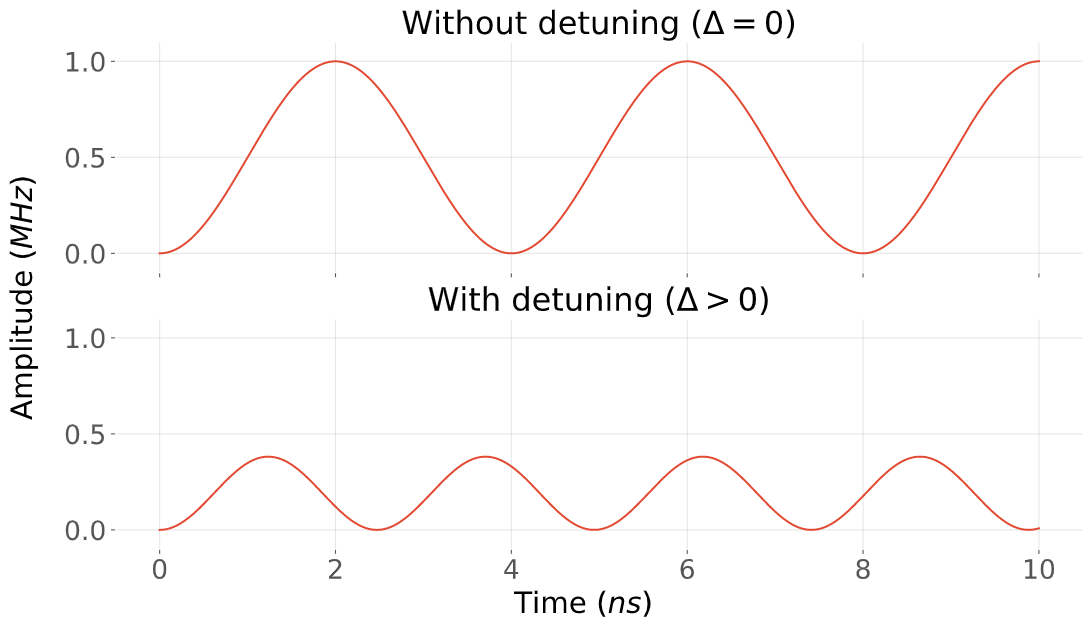
\includegraphics[width=1.0\columnwidth]{gfx/Rabi-Oscilations.png}
%     \caption{Rabi oscillations of atom in a classical electromagnetic field. The top graph is without detuning $\Delta = 0$ and the bottom graph is with detuning $\Delta \ne 0$}
%     \label{fig:rabi-oscillations}
% \end{figure}
\begin{figure}[H]
    \begin{center}
        %% Creator: Matplotlib, PGF backend
%%
%% To include the figure in your LaTeX document, write
%%   \input{<filename>.pgf}
%%
%% Make sure the required packages are loaded in your preamble
%%   \usepackage{pgf}
%%
%% and, on pdftex
%%   \usepackage[utf8]{inputenc}\DeclareUnicodeCharacter{2212}{-}
%%
%% or, on luatex and xetex
%%   \usepackage{unicode-math}
%%
%% Figures using additional raster images can only be included by \input if
%% they are in the same directory as the main LaTeX file. For loading figures
%% from other directories you can use the `import` package
%%   \usepackage{import}
%%
%% and then include the figures with
%%   \import{<path to file>}{<filename>.pgf}
%%
%% Matplotlib used the following preamble
%%
\begingroup%
\makeatletter%
\begin{pgfpicture}%
\pgfpathrectangle{\pgfpointorigin}{\pgfqpoint{4.650000in}{2.800000in}}%
\pgfusepath{use as bounding box, clip}%
\begin{pgfscope}%
\pgfsetbuttcap%
\pgfsetmiterjoin%
\definecolor{currentfill}{rgb}{1.000000,1.000000,1.000000}%
\pgfsetfillcolor{currentfill}%
\pgfsetlinewidth{0.000000pt}%
\definecolor{currentstroke}{rgb}{1.000000,1.000000,1.000000}%
\pgfsetstrokecolor{currentstroke}%
\pgfsetdash{}{0pt}%
\pgfpathmoveto{\pgfqpoint{0.000000in}{0.000000in}}%
\pgfpathlineto{\pgfqpoint{4.650000in}{0.000000in}}%
\pgfpathlineto{\pgfqpoint{4.650000in}{2.800000in}}%
\pgfpathlineto{\pgfqpoint{0.000000in}{2.800000in}}%
\pgfpathclose%
\pgfusepath{fill}%
\end{pgfscope}%
\begin{pgfscope}%
\pgfsetbuttcap%
\pgfsetmiterjoin%
\definecolor{currentfill}{rgb}{1.000000,1.000000,1.000000}%
\pgfsetfillcolor{currentfill}%
\pgfsetlinewidth{0.000000pt}%
\definecolor{currentstroke}{rgb}{0.000000,0.000000,0.000000}%
\pgfsetstrokecolor{currentstroke}%
\pgfsetstrokeopacity{0.000000}%
\pgfsetdash{}{0pt}%
\pgfpathmoveto{\pgfqpoint{0.581250in}{1.544870in}}%
\pgfpathlineto{\pgfqpoint{4.185000in}{1.544870in}}%
\pgfpathlineto{\pgfqpoint{4.185000in}{2.464000in}}%
\pgfpathlineto{\pgfqpoint{0.581250in}{2.464000in}}%
\pgfpathclose%
\pgfusepath{fill}%
\end{pgfscope}%
\begin{pgfscope}%
\pgfpathrectangle{\pgfqpoint{0.581250in}{1.544870in}}{\pgfqpoint{3.603750in}{0.919130in}}%
\pgfusepath{clip}%
\pgfsetrectcap%
\pgfsetroundjoin%
\pgfsetlinewidth{0.803000pt}%
\definecolor{currentstroke}{rgb}{0.501961,0.501961,0.501961}%
\pgfsetstrokecolor{currentstroke}%
\pgfsetstrokeopacity{0.200000}%
\pgfsetdash{}{0pt}%
\pgfpathmoveto{\pgfqpoint{0.745057in}{1.544870in}}%
\pgfpathlineto{\pgfqpoint{0.745057in}{2.464000in}}%
\pgfusepath{stroke}%
\end{pgfscope}%
\begin{pgfscope}%
\pgfsetbuttcap%
\pgfsetroundjoin%
\definecolor{currentfill}{rgb}{0.333333,0.333333,0.333333}%
\pgfsetfillcolor{currentfill}%
\pgfsetlinewidth{0.803000pt}%
\definecolor{currentstroke}{rgb}{0.333333,0.333333,0.333333}%
\pgfsetstrokecolor{currentstroke}%
\pgfsetdash{}{0pt}%
\pgfsys@defobject{currentmarker}{\pgfqpoint{0.000000in}{-0.048611in}}{\pgfqpoint{0.000000in}{0.000000in}}{%
\pgfpathmoveto{\pgfqpoint{0.000000in}{0.000000in}}%
\pgfpathlineto{\pgfqpoint{0.000000in}{-0.048611in}}%
\pgfusepath{stroke,fill}%
}%
\begin{pgfscope}%
\pgfsys@transformshift{0.745057in}{1.544870in}%
\pgfsys@useobject{currentmarker}{}%
\end{pgfscope}%
\end{pgfscope}%
\begin{pgfscope}%
\pgfpathrectangle{\pgfqpoint{0.581250in}{1.544870in}}{\pgfqpoint{3.603750in}{0.919130in}}%
\pgfusepath{clip}%
\pgfsetrectcap%
\pgfsetroundjoin%
\pgfsetlinewidth{0.803000pt}%
\definecolor{currentstroke}{rgb}{0.501961,0.501961,0.501961}%
\pgfsetstrokecolor{currentstroke}%
\pgfsetstrokeopacity{0.200000}%
\pgfsetdash{}{0pt}%
\pgfpathmoveto{\pgfqpoint{1.400284in}{1.544870in}}%
\pgfpathlineto{\pgfqpoint{1.400284in}{2.464000in}}%
\pgfusepath{stroke}%
\end{pgfscope}%
\begin{pgfscope}%
\pgfsetbuttcap%
\pgfsetroundjoin%
\definecolor{currentfill}{rgb}{0.333333,0.333333,0.333333}%
\pgfsetfillcolor{currentfill}%
\pgfsetlinewidth{0.803000pt}%
\definecolor{currentstroke}{rgb}{0.333333,0.333333,0.333333}%
\pgfsetstrokecolor{currentstroke}%
\pgfsetdash{}{0pt}%
\pgfsys@defobject{currentmarker}{\pgfqpoint{0.000000in}{-0.048611in}}{\pgfqpoint{0.000000in}{0.000000in}}{%
\pgfpathmoveto{\pgfqpoint{0.000000in}{0.000000in}}%
\pgfpathlineto{\pgfqpoint{0.000000in}{-0.048611in}}%
\pgfusepath{stroke,fill}%
}%
\begin{pgfscope}%
\pgfsys@transformshift{1.400284in}{1.544870in}%
\pgfsys@useobject{currentmarker}{}%
\end{pgfscope}%
\end{pgfscope}%
\begin{pgfscope}%
\pgfpathrectangle{\pgfqpoint{0.581250in}{1.544870in}}{\pgfqpoint{3.603750in}{0.919130in}}%
\pgfusepath{clip}%
\pgfsetrectcap%
\pgfsetroundjoin%
\pgfsetlinewidth{0.803000pt}%
\definecolor{currentstroke}{rgb}{0.501961,0.501961,0.501961}%
\pgfsetstrokecolor{currentstroke}%
\pgfsetstrokeopacity{0.200000}%
\pgfsetdash{}{0pt}%
\pgfpathmoveto{\pgfqpoint{2.055511in}{1.544870in}}%
\pgfpathlineto{\pgfqpoint{2.055511in}{2.464000in}}%
\pgfusepath{stroke}%
\end{pgfscope}%
\begin{pgfscope}%
\pgfsetbuttcap%
\pgfsetroundjoin%
\definecolor{currentfill}{rgb}{0.333333,0.333333,0.333333}%
\pgfsetfillcolor{currentfill}%
\pgfsetlinewidth{0.803000pt}%
\definecolor{currentstroke}{rgb}{0.333333,0.333333,0.333333}%
\pgfsetstrokecolor{currentstroke}%
\pgfsetdash{}{0pt}%
\pgfsys@defobject{currentmarker}{\pgfqpoint{0.000000in}{-0.048611in}}{\pgfqpoint{0.000000in}{0.000000in}}{%
\pgfpathmoveto{\pgfqpoint{0.000000in}{0.000000in}}%
\pgfpathlineto{\pgfqpoint{0.000000in}{-0.048611in}}%
\pgfusepath{stroke,fill}%
}%
\begin{pgfscope}%
\pgfsys@transformshift{2.055511in}{1.544870in}%
\pgfsys@useobject{currentmarker}{}%
\end{pgfscope}%
\end{pgfscope}%
\begin{pgfscope}%
\pgfpathrectangle{\pgfqpoint{0.581250in}{1.544870in}}{\pgfqpoint{3.603750in}{0.919130in}}%
\pgfusepath{clip}%
\pgfsetrectcap%
\pgfsetroundjoin%
\pgfsetlinewidth{0.803000pt}%
\definecolor{currentstroke}{rgb}{0.501961,0.501961,0.501961}%
\pgfsetstrokecolor{currentstroke}%
\pgfsetstrokeopacity{0.200000}%
\pgfsetdash{}{0pt}%
\pgfpathmoveto{\pgfqpoint{2.710739in}{1.544870in}}%
\pgfpathlineto{\pgfqpoint{2.710739in}{2.464000in}}%
\pgfusepath{stroke}%
\end{pgfscope}%
\begin{pgfscope}%
\pgfsetbuttcap%
\pgfsetroundjoin%
\definecolor{currentfill}{rgb}{0.333333,0.333333,0.333333}%
\pgfsetfillcolor{currentfill}%
\pgfsetlinewidth{0.803000pt}%
\definecolor{currentstroke}{rgb}{0.333333,0.333333,0.333333}%
\pgfsetstrokecolor{currentstroke}%
\pgfsetdash{}{0pt}%
\pgfsys@defobject{currentmarker}{\pgfqpoint{0.000000in}{-0.048611in}}{\pgfqpoint{0.000000in}{0.000000in}}{%
\pgfpathmoveto{\pgfqpoint{0.000000in}{0.000000in}}%
\pgfpathlineto{\pgfqpoint{0.000000in}{-0.048611in}}%
\pgfusepath{stroke,fill}%
}%
\begin{pgfscope}%
\pgfsys@transformshift{2.710739in}{1.544870in}%
\pgfsys@useobject{currentmarker}{}%
\end{pgfscope}%
\end{pgfscope}%
\begin{pgfscope}%
\pgfpathrectangle{\pgfqpoint{0.581250in}{1.544870in}}{\pgfqpoint{3.603750in}{0.919130in}}%
\pgfusepath{clip}%
\pgfsetrectcap%
\pgfsetroundjoin%
\pgfsetlinewidth{0.803000pt}%
\definecolor{currentstroke}{rgb}{0.501961,0.501961,0.501961}%
\pgfsetstrokecolor{currentstroke}%
\pgfsetstrokeopacity{0.200000}%
\pgfsetdash{}{0pt}%
\pgfpathmoveto{\pgfqpoint{3.365966in}{1.544870in}}%
\pgfpathlineto{\pgfqpoint{3.365966in}{2.464000in}}%
\pgfusepath{stroke}%
\end{pgfscope}%
\begin{pgfscope}%
\pgfsetbuttcap%
\pgfsetroundjoin%
\definecolor{currentfill}{rgb}{0.333333,0.333333,0.333333}%
\pgfsetfillcolor{currentfill}%
\pgfsetlinewidth{0.803000pt}%
\definecolor{currentstroke}{rgb}{0.333333,0.333333,0.333333}%
\pgfsetstrokecolor{currentstroke}%
\pgfsetdash{}{0pt}%
\pgfsys@defobject{currentmarker}{\pgfqpoint{0.000000in}{-0.048611in}}{\pgfqpoint{0.000000in}{0.000000in}}{%
\pgfpathmoveto{\pgfqpoint{0.000000in}{0.000000in}}%
\pgfpathlineto{\pgfqpoint{0.000000in}{-0.048611in}}%
\pgfusepath{stroke,fill}%
}%
\begin{pgfscope}%
\pgfsys@transformshift{3.365966in}{1.544870in}%
\pgfsys@useobject{currentmarker}{}%
\end{pgfscope}%
\end{pgfscope}%
\begin{pgfscope}%
\pgfpathrectangle{\pgfqpoint{0.581250in}{1.544870in}}{\pgfqpoint{3.603750in}{0.919130in}}%
\pgfusepath{clip}%
\pgfsetrectcap%
\pgfsetroundjoin%
\pgfsetlinewidth{0.803000pt}%
\definecolor{currentstroke}{rgb}{0.501961,0.501961,0.501961}%
\pgfsetstrokecolor{currentstroke}%
\pgfsetstrokeopacity{0.200000}%
\pgfsetdash{}{0pt}%
\pgfpathmoveto{\pgfqpoint{4.021193in}{1.544870in}}%
\pgfpathlineto{\pgfqpoint{4.021193in}{2.464000in}}%
\pgfusepath{stroke}%
\end{pgfscope}%
\begin{pgfscope}%
\pgfsetbuttcap%
\pgfsetroundjoin%
\definecolor{currentfill}{rgb}{0.333333,0.333333,0.333333}%
\pgfsetfillcolor{currentfill}%
\pgfsetlinewidth{0.803000pt}%
\definecolor{currentstroke}{rgb}{0.333333,0.333333,0.333333}%
\pgfsetstrokecolor{currentstroke}%
\pgfsetdash{}{0pt}%
\pgfsys@defobject{currentmarker}{\pgfqpoint{0.000000in}{-0.048611in}}{\pgfqpoint{0.000000in}{0.000000in}}{%
\pgfpathmoveto{\pgfqpoint{0.000000in}{0.000000in}}%
\pgfpathlineto{\pgfqpoint{0.000000in}{-0.048611in}}%
\pgfusepath{stroke,fill}%
}%
\begin{pgfscope}%
\pgfsys@transformshift{4.021193in}{1.544870in}%
\pgfsys@useobject{currentmarker}{}%
\end{pgfscope}%
\end{pgfscope}%
\begin{pgfscope}%
\pgfpathrectangle{\pgfqpoint{0.581250in}{1.544870in}}{\pgfqpoint{3.603750in}{0.919130in}}%
\pgfusepath{clip}%
\pgfsetrectcap%
\pgfsetroundjoin%
\pgfsetlinewidth{0.803000pt}%
\definecolor{currentstroke}{rgb}{0.501961,0.501961,0.501961}%
\pgfsetstrokecolor{currentstroke}%
\pgfsetstrokeopacity{0.200000}%
\pgfsetdash{}{0pt}%
\pgfpathmoveto{\pgfqpoint{0.581250in}{1.621464in}}%
\pgfpathlineto{\pgfqpoint{4.185000in}{1.621464in}}%
\pgfusepath{stroke}%
\end{pgfscope}%
\begin{pgfscope}%
\pgfsetbuttcap%
\pgfsetroundjoin%
\definecolor{currentfill}{rgb}{0.333333,0.333333,0.333333}%
\pgfsetfillcolor{currentfill}%
\pgfsetlinewidth{0.803000pt}%
\definecolor{currentstroke}{rgb}{0.333333,0.333333,0.333333}%
\pgfsetstrokecolor{currentstroke}%
\pgfsetdash{}{0pt}%
\pgfsys@defobject{currentmarker}{\pgfqpoint{-0.048611in}{0.000000in}}{\pgfqpoint{0.000000in}{0.000000in}}{%
\pgfpathmoveto{\pgfqpoint{0.000000in}{0.000000in}}%
\pgfpathlineto{\pgfqpoint{-0.048611in}{0.000000in}}%
\pgfusepath{stroke,fill}%
}%
\begin{pgfscope}%
\pgfsys@transformshift{0.581250in}{1.621464in}%
\pgfsys@useobject{currentmarker}{}%
\end{pgfscope}%
\end{pgfscope}%
\begin{pgfscope}%
\definecolor{textcolor}{rgb}{0.333333,0.333333,0.333333}%
\pgfsetstrokecolor{textcolor}%
\pgfsetfillcolor{textcolor}%
\pgftext[x=0.414583in, y=1.573238in, left, base]{\color{textcolor}\rmfamily\fontsize{10.000000}{12.000000}\selectfont \(\displaystyle {0}\)}%
\end{pgfscope}%
\begin{pgfscope}%
\pgfpathrectangle{\pgfqpoint{0.581250in}{1.544870in}}{\pgfqpoint{3.603750in}{0.919130in}}%
\pgfusepath{clip}%
\pgfsetrectcap%
\pgfsetroundjoin%
\pgfsetlinewidth{0.803000pt}%
\definecolor{currentstroke}{rgb}{0.501961,0.501961,0.501961}%
\pgfsetstrokecolor{currentstroke}%
\pgfsetstrokeopacity{0.200000}%
\pgfsetdash{}{0pt}%
\pgfpathmoveto{\pgfqpoint{0.581250in}{2.387406in}}%
\pgfpathlineto{\pgfqpoint{4.185000in}{2.387406in}}%
\pgfusepath{stroke}%
\end{pgfscope}%
\begin{pgfscope}%
\pgfsetbuttcap%
\pgfsetroundjoin%
\definecolor{currentfill}{rgb}{0.333333,0.333333,0.333333}%
\pgfsetfillcolor{currentfill}%
\pgfsetlinewidth{0.803000pt}%
\definecolor{currentstroke}{rgb}{0.333333,0.333333,0.333333}%
\pgfsetstrokecolor{currentstroke}%
\pgfsetdash{}{0pt}%
\pgfsys@defobject{currentmarker}{\pgfqpoint{-0.048611in}{0.000000in}}{\pgfqpoint{0.000000in}{0.000000in}}{%
\pgfpathmoveto{\pgfqpoint{0.000000in}{0.000000in}}%
\pgfpathlineto{\pgfqpoint{-0.048611in}{0.000000in}}%
\pgfusepath{stroke,fill}%
}%
\begin{pgfscope}%
\pgfsys@transformshift{0.581250in}{2.387406in}%
\pgfsys@useobject{currentmarker}{}%
\end{pgfscope}%
\end{pgfscope}%
\begin{pgfscope}%
\definecolor{textcolor}{rgb}{0.333333,0.333333,0.333333}%
\pgfsetstrokecolor{textcolor}%
\pgfsetfillcolor{textcolor}%
\pgftext[x=0.414583in, y=2.339181in, left, base]{\color{textcolor}\rmfamily\fontsize{10.000000}{12.000000}\selectfont \(\displaystyle {1}\)}%
\end{pgfscope}%
\begin{pgfscope}%
\pgfpathrectangle{\pgfqpoint{0.581250in}{1.544870in}}{\pgfqpoint{3.603750in}{0.919130in}}%
\pgfusepath{clip}%
\pgfsetrectcap%
\pgfsetroundjoin%
\pgfsetlinewidth{1.505625pt}%
\definecolor{currentstroke}{rgb}{0.886275,0.290196,0.200000}%
\pgfsetstrokecolor{currentstroke}%
\pgfsetdash{}{0pt}%
\pgfpathmoveto{\pgfqpoint{0.745057in}{1.621464in}}%
\pgfpathlineto{\pgfqpoint{0.778149in}{1.626274in}}%
\pgfpathlineto{\pgfqpoint{0.811241in}{1.640585in}}%
\pgfpathlineto{\pgfqpoint{0.844334in}{1.664037in}}%
\pgfpathlineto{\pgfqpoint{0.877426in}{1.696040in}}%
\pgfpathlineto{\pgfqpoint{0.910518in}{1.735790in}}%
\pgfpathlineto{\pgfqpoint{0.943611in}{1.782290in}}%
\pgfpathlineto{\pgfqpoint{0.976703in}{1.834370in}}%
\pgfpathlineto{\pgfqpoint{1.009795in}{1.890723in}}%
\pgfpathlineto{\pgfqpoint{1.042887in}{1.949932in}}%
\pgfpathlineto{\pgfqpoint{1.075980in}{2.010511in}}%
\pgfpathlineto{\pgfqpoint{1.109072in}{2.070937in}}%
\pgfpathlineto{\pgfqpoint{1.142164in}{2.129692in}}%
\pgfpathlineto{\pgfqpoint{1.175257in}{2.185301in}}%
\pgfpathlineto{\pgfqpoint{1.208349in}{2.236366in}}%
\pgfpathlineto{\pgfqpoint{1.241441in}{2.281604in}}%
\pgfpathlineto{\pgfqpoint{1.274533in}{2.319879in}}%
\pgfpathlineto{\pgfqpoint{1.307626in}{2.350229in}}%
\pgfpathlineto{\pgfqpoint{1.340718in}{2.371893in}}%
\pgfpathlineto{\pgfqpoint{1.373810in}{2.384325in}}%
\pgfpathlineto{\pgfqpoint{1.406903in}{2.387213in}}%
\pgfpathlineto{\pgfqpoint{1.439995in}{2.380485in}}%
\pgfpathlineto{\pgfqpoint{1.473087in}{2.364310in}}%
\pgfpathlineto{\pgfqpoint{1.506179in}{2.339094in}}%
\pgfpathlineto{\pgfqpoint{1.539272in}{2.305470in}}%
\pgfpathlineto{\pgfqpoint{1.572364in}{2.264284in}}%
\pgfpathlineto{\pgfqpoint{1.605456in}{2.216570in}}%
\pgfpathlineto{\pgfqpoint{1.638549in}{2.163527in}}%
\pgfpathlineto{\pgfqpoint{1.671641in}{2.106487in}}%
\pgfpathlineto{\pgfqpoint{1.704733in}{2.046883in}}%
\pgfpathlineto{\pgfqpoint{1.737825in}{1.986212in}}%
\pgfpathlineto{\pgfqpoint{1.770918in}{1.926000in}}%
\pgfpathlineto{\pgfqpoint{1.804010in}{1.867758in}}%
\pgfpathlineto{\pgfqpoint{1.837102in}{1.812949in}}%
\pgfpathlineto{\pgfqpoint{1.870195in}{1.762951in}}%
\pgfpathlineto{\pgfqpoint{1.903287in}{1.719020in}}%
\pgfpathlineto{\pgfqpoint{1.936379in}{1.682259in}}%
\pgfpathlineto{\pgfqpoint{1.969471in}{1.653592in}}%
\pgfpathlineto{\pgfqpoint{2.002564in}{1.633738in}}%
\pgfpathlineto{\pgfqpoint{2.035656in}{1.623198in}}%
\pgfpathlineto{\pgfqpoint{2.068748in}{1.622235in}}%
\pgfpathlineto{\pgfqpoint{2.101841in}{1.630873in}}%
\pgfpathlineto{\pgfqpoint{2.134933in}{1.648897in}}%
\pgfpathlineto{\pgfqpoint{2.168025in}{1.675852in}}%
\pgfpathlineto{\pgfqpoint{2.201117in}{1.711062in}}%
\pgfpathlineto{\pgfqpoint{2.234210in}{1.753642in}}%
\pgfpathlineto{\pgfqpoint{2.267302in}{1.802523in}}%
\pgfpathlineto{\pgfqpoint{2.300394in}{1.856476in}}%
\pgfpathlineto{\pgfqpoint{2.333487in}{1.914146in}}%
\pgfpathlineto{\pgfqpoint{2.366579in}{1.974084in}}%
\pgfpathlineto{\pgfqpoint{2.399671in}{2.034785in}}%
\pgfpathlineto{\pgfqpoint{2.432763in}{2.094724in}}%
\pgfpathlineto{\pgfqpoint{2.465856in}{2.152394in}}%
\pgfpathlineto{\pgfqpoint{2.498948in}{2.206347in}}%
\pgfpathlineto{\pgfqpoint{2.532040in}{2.255227in}}%
\pgfpathlineto{\pgfqpoint{2.565133in}{2.297808in}}%
\pgfpathlineto{\pgfqpoint{2.598225in}{2.333018in}}%
\pgfpathlineto{\pgfqpoint{2.631317in}{2.359973in}}%
\pgfpathlineto{\pgfqpoint{2.664409in}{2.377996in}}%
\pgfpathlineto{\pgfqpoint{2.697502in}{2.386635in}}%
\pgfpathlineto{\pgfqpoint{2.730594in}{2.385672in}}%
\pgfpathlineto{\pgfqpoint{2.763686in}{2.375131in}}%
\pgfpathlineto{\pgfqpoint{2.796779in}{2.355278in}}%
\pgfpathlineto{\pgfqpoint{2.829871in}{2.326611in}}%
\pgfpathlineto{\pgfqpoint{2.862963in}{2.289849in}}%
\pgfpathlineto{\pgfqpoint{2.896055in}{2.245918in}}%
\pgfpathlineto{\pgfqpoint{2.929148in}{2.195920in}}%
\pgfpathlineto{\pgfqpoint{2.962240in}{2.141112in}}%
\pgfpathlineto{\pgfqpoint{2.995332in}{2.082870in}}%
\pgfpathlineto{\pgfqpoint{3.028425in}{2.022657in}}%
\pgfpathlineto{\pgfqpoint{3.061517in}{1.961987in}}%
\pgfpathlineto{\pgfqpoint{3.094609in}{1.902383in}}%
\pgfpathlineto{\pgfqpoint{3.127701in}{1.845343in}}%
\pgfpathlineto{\pgfqpoint{3.160794in}{1.792299in}}%
\pgfpathlineto{\pgfqpoint{3.193886in}{1.744585in}}%
\pgfpathlineto{\pgfqpoint{3.226978in}{1.703399in}}%
\pgfpathlineto{\pgfqpoint{3.260071in}{1.669776in}}%
\pgfpathlineto{\pgfqpoint{3.293163in}{1.644560in}}%
\pgfpathlineto{\pgfqpoint{3.326255in}{1.628385in}}%
\pgfpathlineto{\pgfqpoint{3.359347in}{1.621657in}}%
\pgfpathlineto{\pgfqpoint{3.392440in}{1.624545in}}%
\pgfpathlineto{\pgfqpoint{3.425532in}{1.636977in}}%
\pgfpathlineto{\pgfqpoint{3.458624in}{1.658640in}}%
\pgfpathlineto{\pgfqpoint{3.491717in}{1.688991in}}%
\pgfpathlineto{\pgfqpoint{3.524809in}{1.727266in}}%
\pgfpathlineto{\pgfqpoint{3.557901in}{1.772504in}}%
\pgfpathlineto{\pgfqpoint{3.590993in}{1.823569in}}%
\pgfpathlineto{\pgfqpoint{3.624086in}{1.879177in}}%
\pgfpathlineto{\pgfqpoint{3.657178in}{1.937933in}}%
\pgfpathlineto{\pgfqpoint{3.690270in}{1.998359in}}%
\pgfpathlineto{\pgfqpoint{3.723363in}{2.058937in}}%
\pgfpathlineto{\pgfqpoint{3.756455in}{2.118147in}}%
\pgfpathlineto{\pgfqpoint{3.789547in}{2.174499in}}%
\pgfpathlineto{\pgfqpoint{3.822639in}{2.226580in}}%
\pgfpathlineto{\pgfqpoint{3.855732in}{2.273079in}}%
\pgfpathlineto{\pgfqpoint{3.888824in}{2.312830in}}%
\pgfpathlineto{\pgfqpoint{3.921916in}{2.344833in}}%
\pgfpathlineto{\pgfqpoint{3.955009in}{2.368284in}}%
\pgfpathlineto{\pgfqpoint{3.988101in}{2.382595in}}%
\pgfpathlineto{\pgfqpoint{4.021193in}{2.387406in}}%
\pgfusepath{stroke}%
\end{pgfscope}%
\begin{pgfscope}%
\pgfsetrectcap%
\pgfsetmiterjoin%
\pgfsetlinewidth{1.003750pt}%
\definecolor{currentstroke}{rgb}{1.000000,1.000000,1.000000}%
\pgfsetstrokecolor{currentstroke}%
\pgfsetdash{}{0pt}%
\pgfpathmoveto{\pgfqpoint{0.581250in}{1.544870in}}%
\pgfpathlineto{\pgfqpoint{0.581250in}{2.464000in}}%
\pgfusepath{stroke}%
\end{pgfscope}%
\begin{pgfscope}%
\pgfsetrectcap%
\pgfsetmiterjoin%
\pgfsetlinewidth{1.003750pt}%
\definecolor{currentstroke}{rgb}{1.000000,1.000000,1.000000}%
\pgfsetstrokecolor{currentstroke}%
\pgfsetdash{}{0pt}%
\pgfpathmoveto{\pgfqpoint{4.185000in}{1.544870in}}%
\pgfpathlineto{\pgfqpoint{4.185000in}{2.464000in}}%
\pgfusepath{stroke}%
\end{pgfscope}%
\begin{pgfscope}%
\pgfsetrectcap%
\pgfsetmiterjoin%
\pgfsetlinewidth{1.003750pt}%
\definecolor{currentstroke}{rgb}{1.000000,1.000000,1.000000}%
\pgfsetstrokecolor{currentstroke}%
\pgfsetdash{}{0pt}%
\pgfpathmoveto{\pgfqpoint{0.581250in}{1.544870in}}%
\pgfpathlineto{\pgfqpoint{4.185000in}{1.544870in}}%
\pgfusepath{stroke}%
\end{pgfscope}%
\begin{pgfscope}%
\pgfsetrectcap%
\pgfsetmiterjoin%
\pgfsetlinewidth{1.003750pt}%
\definecolor{currentstroke}{rgb}{1.000000,1.000000,1.000000}%
\pgfsetstrokecolor{currentstroke}%
\pgfsetdash{}{0pt}%
\pgfpathmoveto{\pgfqpoint{0.581250in}{2.464000in}}%
\pgfpathlineto{\pgfqpoint{4.185000in}{2.464000in}}%
\pgfusepath{stroke}%
\end{pgfscope}%
\begin{pgfscope}%
\definecolor{textcolor}{rgb}{0.000000,0.000000,0.000000}%
\pgfsetstrokecolor{textcolor}%
\pgfsetfillcolor{textcolor}%
\pgftext[x=2.383125in,y=2.547333in,,base]{\color{textcolor}\rmfamily\fontsize{14.000000}{16.800000}\selectfont Without detuning (\(\displaystyle \Delta=0\))}%
\end{pgfscope}%
\begin{pgfscope}%
\pgfsetbuttcap%
\pgfsetmiterjoin%
\definecolor{currentfill}{rgb}{1.000000,1.000000,1.000000}%
\pgfsetfillcolor{currentfill}%
\pgfsetlinewidth{0.000000pt}%
\definecolor{currentstroke}{rgb}{0.000000,0.000000,0.000000}%
\pgfsetstrokecolor{currentstroke}%
\pgfsetstrokeopacity{0.000000}%
\pgfsetdash{}{0pt}%
\pgfpathmoveto{\pgfqpoint{0.581250in}{0.350000in}}%
\pgfpathlineto{\pgfqpoint{4.185000in}{0.350000in}}%
\pgfpathlineto{\pgfqpoint{4.185000in}{1.269130in}}%
\pgfpathlineto{\pgfqpoint{0.581250in}{1.269130in}}%
\pgfpathclose%
\pgfusepath{fill}%
\end{pgfscope}%
\begin{pgfscope}%
\pgfpathrectangle{\pgfqpoint{0.581250in}{0.350000in}}{\pgfqpoint{3.603750in}{0.919130in}}%
\pgfusepath{clip}%
\pgfsetrectcap%
\pgfsetroundjoin%
\pgfsetlinewidth{0.803000pt}%
\definecolor{currentstroke}{rgb}{0.501961,0.501961,0.501961}%
\pgfsetstrokecolor{currentstroke}%
\pgfsetstrokeopacity{0.200000}%
\pgfsetdash{}{0pt}%
\pgfpathmoveto{\pgfqpoint{0.745057in}{0.350000in}}%
\pgfpathlineto{\pgfqpoint{0.745057in}{1.269130in}}%
\pgfusepath{stroke}%
\end{pgfscope}%
\begin{pgfscope}%
\pgfsetbuttcap%
\pgfsetroundjoin%
\definecolor{currentfill}{rgb}{0.333333,0.333333,0.333333}%
\pgfsetfillcolor{currentfill}%
\pgfsetlinewidth{0.803000pt}%
\definecolor{currentstroke}{rgb}{0.333333,0.333333,0.333333}%
\pgfsetstrokecolor{currentstroke}%
\pgfsetdash{}{0pt}%
\pgfsys@defobject{currentmarker}{\pgfqpoint{0.000000in}{-0.048611in}}{\pgfqpoint{0.000000in}{0.000000in}}{%
\pgfpathmoveto{\pgfqpoint{0.000000in}{0.000000in}}%
\pgfpathlineto{\pgfqpoint{0.000000in}{-0.048611in}}%
\pgfusepath{stroke,fill}%
}%
\begin{pgfscope}%
\pgfsys@transformshift{0.745057in}{0.350000in}%
\pgfsys@useobject{currentmarker}{}%
\end{pgfscope}%
\end{pgfscope}%
\begin{pgfscope}%
\definecolor{textcolor}{rgb}{0.333333,0.333333,0.333333}%
\pgfsetstrokecolor{textcolor}%
\pgfsetfillcolor{textcolor}%
\pgftext[x=0.745057in,y=0.252778in,,top]{\color{textcolor}\rmfamily\fontsize{10.000000}{12.000000}\selectfont \(\displaystyle {0}\)}%
\end{pgfscope}%
\begin{pgfscope}%
\pgfpathrectangle{\pgfqpoint{0.581250in}{0.350000in}}{\pgfqpoint{3.603750in}{0.919130in}}%
\pgfusepath{clip}%
\pgfsetrectcap%
\pgfsetroundjoin%
\pgfsetlinewidth{0.803000pt}%
\definecolor{currentstroke}{rgb}{0.501961,0.501961,0.501961}%
\pgfsetstrokecolor{currentstroke}%
\pgfsetstrokeopacity{0.200000}%
\pgfsetdash{}{0pt}%
\pgfpathmoveto{\pgfqpoint{1.400284in}{0.350000in}}%
\pgfpathlineto{\pgfqpoint{1.400284in}{1.269130in}}%
\pgfusepath{stroke}%
\end{pgfscope}%
\begin{pgfscope}%
\pgfsetbuttcap%
\pgfsetroundjoin%
\definecolor{currentfill}{rgb}{0.333333,0.333333,0.333333}%
\pgfsetfillcolor{currentfill}%
\pgfsetlinewidth{0.803000pt}%
\definecolor{currentstroke}{rgb}{0.333333,0.333333,0.333333}%
\pgfsetstrokecolor{currentstroke}%
\pgfsetdash{}{0pt}%
\pgfsys@defobject{currentmarker}{\pgfqpoint{0.000000in}{-0.048611in}}{\pgfqpoint{0.000000in}{0.000000in}}{%
\pgfpathmoveto{\pgfqpoint{0.000000in}{0.000000in}}%
\pgfpathlineto{\pgfqpoint{0.000000in}{-0.048611in}}%
\pgfusepath{stroke,fill}%
}%
\begin{pgfscope}%
\pgfsys@transformshift{1.400284in}{0.350000in}%
\pgfsys@useobject{currentmarker}{}%
\end{pgfscope}%
\end{pgfscope}%
\begin{pgfscope}%
\definecolor{textcolor}{rgb}{0.333333,0.333333,0.333333}%
\pgfsetstrokecolor{textcolor}%
\pgfsetfillcolor{textcolor}%
\pgftext[x=1.400284in,y=0.252778in,,top]{\color{textcolor}\rmfamily\fontsize{10.000000}{12.000000}\selectfont \(\displaystyle {2}\)}%
\end{pgfscope}%
\begin{pgfscope}%
\pgfpathrectangle{\pgfqpoint{0.581250in}{0.350000in}}{\pgfqpoint{3.603750in}{0.919130in}}%
\pgfusepath{clip}%
\pgfsetrectcap%
\pgfsetroundjoin%
\pgfsetlinewidth{0.803000pt}%
\definecolor{currentstroke}{rgb}{0.501961,0.501961,0.501961}%
\pgfsetstrokecolor{currentstroke}%
\pgfsetstrokeopacity{0.200000}%
\pgfsetdash{}{0pt}%
\pgfpathmoveto{\pgfqpoint{2.055511in}{0.350000in}}%
\pgfpathlineto{\pgfqpoint{2.055511in}{1.269130in}}%
\pgfusepath{stroke}%
\end{pgfscope}%
\begin{pgfscope}%
\pgfsetbuttcap%
\pgfsetroundjoin%
\definecolor{currentfill}{rgb}{0.333333,0.333333,0.333333}%
\pgfsetfillcolor{currentfill}%
\pgfsetlinewidth{0.803000pt}%
\definecolor{currentstroke}{rgb}{0.333333,0.333333,0.333333}%
\pgfsetstrokecolor{currentstroke}%
\pgfsetdash{}{0pt}%
\pgfsys@defobject{currentmarker}{\pgfqpoint{0.000000in}{-0.048611in}}{\pgfqpoint{0.000000in}{0.000000in}}{%
\pgfpathmoveto{\pgfqpoint{0.000000in}{0.000000in}}%
\pgfpathlineto{\pgfqpoint{0.000000in}{-0.048611in}}%
\pgfusepath{stroke,fill}%
}%
\begin{pgfscope}%
\pgfsys@transformshift{2.055511in}{0.350000in}%
\pgfsys@useobject{currentmarker}{}%
\end{pgfscope}%
\end{pgfscope}%
\begin{pgfscope}%
\definecolor{textcolor}{rgb}{0.333333,0.333333,0.333333}%
\pgfsetstrokecolor{textcolor}%
\pgfsetfillcolor{textcolor}%
\pgftext[x=2.055511in,y=0.252778in,,top]{\color{textcolor}\rmfamily\fontsize{10.000000}{12.000000}\selectfont \(\displaystyle {4}\)}%
\end{pgfscope}%
\begin{pgfscope}%
\pgfpathrectangle{\pgfqpoint{0.581250in}{0.350000in}}{\pgfqpoint{3.603750in}{0.919130in}}%
\pgfusepath{clip}%
\pgfsetrectcap%
\pgfsetroundjoin%
\pgfsetlinewidth{0.803000pt}%
\definecolor{currentstroke}{rgb}{0.501961,0.501961,0.501961}%
\pgfsetstrokecolor{currentstroke}%
\pgfsetstrokeopacity{0.200000}%
\pgfsetdash{}{0pt}%
\pgfpathmoveto{\pgfqpoint{2.710739in}{0.350000in}}%
\pgfpathlineto{\pgfqpoint{2.710739in}{1.269130in}}%
\pgfusepath{stroke}%
\end{pgfscope}%
\begin{pgfscope}%
\pgfsetbuttcap%
\pgfsetroundjoin%
\definecolor{currentfill}{rgb}{0.333333,0.333333,0.333333}%
\pgfsetfillcolor{currentfill}%
\pgfsetlinewidth{0.803000pt}%
\definecolor{currentstroke}{rgb}{0.333333,0.333333,0.333333}%
\pgfsetstrokecolor{currentstroke}%
\pgfsetdash{}{0pt}%
\pgfsys@defobject{currentmarker}{\pgfqpoint{0.000000in}{-0.048611in}}{\pgfqpoint{0.000000in}{0.000000in}}{%
\pgfpathmoveto{\pgfqpoint{0.000000in}{0.000000in}}%
\pgfpathlineto{\pgfqpoint{0.000000in}{-0.048611in}}%
\pgfusepath{stroke,fill}%
}%
\begin{pgfscope}%
\pgfsys@transformshift{2.710739in}{0.350000in}%
\pgfsys@useobject{currentmarker}{}%
\end{pgfscope}%
\end{pgfscope}%
\begin{pgfscope}%
\definecolor{textcolor}{rgb}{0.333333,0.333333,0.333333}%
\pgfsetstrokecolor{textcolor}%
\pgfsetfillcolor{textcolor}%
\pgftext[x=2.710739in,y=0.252778in,,top]{\color{textcolor}\rmfamily\fontsize{10.000000}{12.000000}\selectfont \(\displaystyle {6}\)}%
\end{pgfscope}%
\begin{pgfscope}%
\pgfpathrectangle{\pgfqpoint{0.581250in}{0.350000in}}{\pgfqpoint{3.603750in}{0.919130in}}%
\pgfusepath{clip}%
\pgfsetrectcap%
\pgfsetroundjoin%
\pgfsetlinewidth{0.803000pt}%
\definecolor{currentstroke}{rgb}{0.501961,0.501961,0.501961}%
\pgfsetstrokecolor{currentstroke}%
\pgfsetstrokeopacity{0.200000}%
\pgfsetdash{}{0pt}%
\pgfpathmoveto{\pgfqpoint{3.365966in}{0.350000in}}%
\pgfpathlineto{\pgfqpoint{3.365966in}{1.269130in}}%
\pgfusepath{stroke}%
\end{pgfscope}%
\begin{pgfscope}%
\pgfsetbuttcap%
\pgfsetroundjoin%
\definecolor{currentfill}{rgb}{0.333333,0.333333,0.333333}%
\pgfsetfillcolor{currentfill}%
\pgfsetlinewidth{0.803000pt}%
\definecolor{currentstroke}{rgb}{0.333333,0.333333,0.333333}%
\pgfsetstrokecolor{currentstroke}%
\pgfsetdash{}{0pt}%
\pgfsys@defobject{currentmarker}{\pgfqpoint{0.000000in}{-0.048611in}}{\pgfqpoint{0.000000in}{0.000000in}}{%
\pgfpathmoveto{\pgfqpoint{0.000000in}{0.000000in}}%
\pgfpathlineto{\pgfqpoint{0.000000in}{-0.048611in}}%
\pgfusepath{stroke,fill}%
}%
\begin{pgfscope}%
\pgfsys@transformshift{3.365966in}{0.350000in}%
\pgfsys@useobject{currentmarker}{}%
\end{pgfscope}%
\end{pgfscope}%
\begin{pgfscope}%
\definecolor{textcolor}{rgb}{0.333333,0.333333,0.333333}%
\pgfsetstrokecolor{textcolor}%
\pgfsetfillcolor{textcolor}%
\pgftext[x=3.365966in,y=0.252778in,,top]{\color{textcolor}\rmfamily\fontsize{10.000000}{12.000000}\selectfont \(\displaystyle {8}\)}%
\end{pgfscope}%
\begin{pgfscope}%
\pgfpathrectangle{\pgfqpoint{0.581250in}{0.350000in}}{\pgfqpoint{3.603750in}{0.919130in}}%
\pgfusepath{clip}%
\pgfsetrectcap%
\pgfsetroundjoin%
\pgfsetlinewidth{0.803000pt}%
\definecolor{currentstroke}{rgb}{0.501961,0.501961,0.501961}%
\pgfsetstrokecolor{currentstroke}%
\pgfsetstrokeopacity{0.200000}%
\pgfsetdash{}{0pt}%
\pgfpathmoveto{\pgfqpoint{4.021193in}{0.350000in}}%
\pgfpathlineto{\pgfqpoint{4.021193in}{1.269130in}}%
\pgfusepath{stroke}%
\end{pgfscope}%
\begin{pgfscope}%
\pgfsetbuttcap%
\pgfsetroundjoin%
\definecolor{currentfill}{rgb}{0.333333,0.333333,0.333333}%
\pgfsetfillcolor{currentfill}%
\pgfsetlinewidth{0.803000pt}%
\definecolor{currentstroke}{rgb}{0.333333,0.333333,0.333333}%
\pgfsetstrokecolor{currentstroke}%
\pgfsetdash{}{0pt}%
\pgfsys@defobject{currentmarker}{\pgfqpoint{0.000000in}{-0.048611in}}{\pgfqpoint{0.000000in}{0.000000in}}{%
\pgfpathmoveto{\pgfqpoint{0.000000in}{0.000000in}}%
\pgfpathlineto{\pgfqpoint{0.000000in}{-0.048611in}}%
\pgfusepath{stroke,fill}%
}%
\begin{pgfscope}%
\pgfsys@transformshift{4.021193in}{0.350000in}%
\pgfsys@useobject{currentmarker}{}%
\end{pgfscope}%
\end{pgfscope}%
\begin{pgfscope}%
\definecolor{textcolor}{rgb}{0.333333,0.333333,0.333333}%
\pgfsetstrokecolor{textcolor}%
\pgfsetfillcolor{textcolor}%
\pgftext[x=4.021193in,y=0.252778in,,top]{\color{textcolor}\rmfamily\fontsize{10.000000}{12.000000}\selectfont \(\displaystyle {10}\)}%
\end{pgfscope}%
\begin{pgfscope}%
\pgfpathrectangle{\pgfqpoint{0.581250in}{0.350000in}}{\pgfqpoint{3.603750in}{0.919130in}}%
\pgfusepath{clip}%
\pgfsetrectcap%
\pgfsetroundjoin%
\pgfsetlinewidth{0.803000pt}%
\definecolor{currentstroke}{rgb}{0.501961,0.501961,0.501961}%
\pgfsetstrokecolor{currentstroke}%
\pgfsetstrokeopacity{0.200000}%
\pgfsetdash{}{0pt}%
\pgfpathmoveto{\pgfqpoint{0.581250in}{0.426594in}}%
\pgfpathlineto{\pgfqpoint{4.185000in}{0.426594in}}%
\pgfusepath{stroke}%
\end{pgfscope}%
\begin{pgfscope}%
\pgfsetbuttcap%
\pgfsetroundjoin%
\definecolor{currentfill}{rgb}{0.333333,0.333333,0.333333}%
\pgfsetfillcolor{currentfill}%
\pgfsetlinewidth{0.803000pt}%
\definecolor{currentstroke}{rgb}{0.333333,0.333333,0.333333}%
\pgfsetstrokecolor{currentstroke}%
\pgfsetdash{}{0pt}%
\pgfsys@defobject{currentmarker}{\pgfqpoint{-0.048611in}{0.000000in}}{\pgfqpoint{0.000000in}{0.000000in}}{%
\pgfpathmoveto{\pgfqpoint{0.000000in}{0.000000in}}%
\pgfpathlineto{\pgfqpoint{-0.048611in}{0.000000in}}%
\pgfusepath{stroke,fill}%
}%
\begin{pgfscope}%
\pgfsys@transformshift{0.581250in}{0.426594in}%
\pgfsys@useobject{currentmarker}{}%
\end{pgfscope}%
\end{pgfscope}%
\begin{pgfscope}%
\definecolor{textcolor}{rgb}{0.333333,0.333333,0.333333}%
\pgfsetstrokecolor{textcolor}%
\pgfsetfillcolor{textcolor}%
\pgftext[x=0.414583in, y=0.378369in, left, base]{\color{textcolor}\rmfamily\fontsize{10.000000}{12.000000}\selectfont \(\displaystyle {0}\)}%
\end{pgfscope}%
\begin{pgfscope}%
\pgfpathrectangle{\pgfqpoint{0.581250in}{0.350000in}}{\pgfqpoint{3.603750in}{0.919130in}}%
\pgfusepath{clip}%
\pgfsetrectcap%
\pgfsetroundjoin%
\pgfsetlinewidth{0.803000pt}%
\definecolor{currentstroke}{rgb}{0.501961,0.501961,0.501961}%
\pgfsetstrokecolor{currentstroke}%
\pgfsetstrokeopacity{0.200000}%
\pgfsetdash{}{0pt}%
\pgfpathmoveto{\pgfqpoint{0.581250in}{1.192536in}}%
\pgfpathlineto{\pgfqpoint{4.185000in}{1.192536in}}%
\pgfusepath{stroke}%
\end{pgfscope}%
\begin{pgfscope}%
\pgfsetbuttcap%
\pgfsetroundjoin%
\definecolor{currentfill}{rgb}{0.333333,0.333333,0.333333}%
\pgfsetfillcolor{currentfill}%
\pgfsetlinewidth{0.803000pt}%
\definecolor{currentstroke}{rgb}{0.333333,0.333333,0.333333}%
\pgfsetstrokecolor{currentstroke}%
\pgfsetdash{}{0pt}%
\pgfsys@defobject{currentmarker}{\pgfqpoint{-0.048611in}{0.000000in}}{\pgfqpoint{0.000000in}{0.000000in}}{%
\pgfpathmoveto{\pgfqpoint{0.000000in}{0.000000in}}%
\pgfpathlineto{\pgfqpoint{-0.048611in}{0.000000in}}%
\pgfusepath{stroke,fill}%
}%
\begin{pgfscope}%
\pgfsys@transformshift{0.581250in}{1.192536in}%
\pgfsys@useobject{currentmarker}{}%
\end{pgfscope}%
\end{pgfscope}%
\begin{pgfscope}%
\definecolor{textcolor}{rgb}{0.333333,0.333333,0.333333}%
\pgfsetstrokecolor{textcolor}%
\pgfsetfillcolor{textcolor}%
\pgftext[x=0.414583in, y=1.144311in, left, base]{\color{textcolor}\rmfamily\fontsize{10.000000}{12.000000}\selectfont \(\displaystyle {1}\)}%
\end{pgfscope}%
\begin{pgfscope}%
\pgfpathrectangle{\pgfqpoint{0.581250in}{0.350000in}}{\pgfqpoint{3.603750in}{0.919130in}}%
\pgfusepath{clip}%
\pgfsetrectcap%
\pgfsetroundjoin%
\pgfsetlinewidth{1.505625pt}%
\definecolor{currentstroke}{rgb}{0.886275,0.290196,0.200000}%
\pgfsetstrokecolor{currentstroke}%
\pgfsetdash{}{0pt}%
\pgfpathmoveto{\pgfqpoint{0.745057in}{0.426594in}}%
\pgfpathlineto{\pgfqpoint{0.778149in}{0.431388in}}%
\pgfpathlineto{\pgfqpoint{0.811241in}{0.445456in}}%
\pgfpathlineto{\pgfqpoint{0.844334in}{0.467875in}}%
\pgfpathlineto{\pgfqpoint{0.877426in}{0.497173in}}%
\pgfpathlineto{\pgfqpoint{0.910518in}{0.531427in}}%
\pgfpathlineto{\pgfqpoint{0.943611in}{0.568391in}}%
\pgfpathlineto{\pgfqpoint{0.976703in}{0.605637in}}%
\pgfpathlineto{\pgfqpoint{1.009795in}{0.640722in}}%
\pgfpathlineto{\pgfqpoint{1.042887in}{0.671343in}}%
\pgfpathlineto{\pgfqpoint{1.075980in}{0.695491in}}%
\pgfpathlineto{\pgfqpoint{1.109072in}{0.711581in}}%
\pgfpathlineto{\pgfqpoint{1.142164in}{0.718557in}}%
\pgfpathlineto{\pgfqpoint{1.175257in}{0.715961in}}%
\pgfpathlineto{\pgfqpoint{1.208349in}{0.703964in}}%
\pgfpathlineto{\pgfqpoint{1.241441in}{0.683353in}}%
\pgfpathlineto{\pgfqpoint{1.274533in}{0.655481in}}%
\pgfpathlineto{\pgfqpoint{1.307626in}{0.622176in}}%
\pgfpathlineto{\pgfqpoint{1.340718in}{0.585625in}}%
\pgfpathlineto{\pgfqpoint{1.373810in}{0.548225in}}%
\pgfpathlineto{\pgfqpoint{1.406903in}{0.512432in}}%
\pgfpathlineto{\pgfqpoint{1.439995in}{0.480594in}}%
\pgfpathlineto{\pgfqpoint{1.473087in}{0.454801in}}%
\pgfpathlineto{\pgfqpoint{1.506179in}{0.436745in}}%
\pgfpathlineto{\pgfqpoint{1.539272in}{0.427611in}}%
\pgfpathlineto{\pgfqpoint{1.572364in}{0.427999in}}%
\pgfpathlineto{\pgfqpoint{1.605456in}{0.437884in}}%
\pgfpathlineto{\pgfqpoint{1.638549in}{0.456615in}}%
\pgfpathlineto{\pgfqpoint{1.671641in}{0.482965in}}%
\pgfpathlineto{\pgfqpoint{1.704733in}{0.515204in}}%
\pgfpathlineto{\pgfqpoint{1.737825in}{0.551217in}}%
\pgfpathlineto{\pgfqpoint{1.770918in}{0.588639in}}%
\pgfpathlineto{\pgfqpoint{1.804010in}{0.625015in}}%
\pgfpathlineto{\pgfqpoint{1.837102in}{0.657959in}}%
\pgfpathlineto{\pgfqpoint{1.870195in}{0.685308in}}%
\pgfpathlineto{\pgfqpoint{1.903287in}{0.705266in}}%
\pgfpathlineto{\pgfqpoint{1.936379in}{0.716526in}}%
\pgfpathlineto{\pgfqpoint{1.969471in}{0.718347in}}%
\pgfpathlineto{\pgfqpoint{2.002564in}{0.710610in}}%
\pgfpathlineto{\pgfqpoint{2.035656in}{0.693823in}}%
\pgfpathlineto{\pgfqpoint{2.068748in}{0.669087in}}%
\pgfpathlineto{\pgfqpoint{2.101841in}{0.638026in}}%
\pgfpathlineto{\pgfqpoint{2.134933in}{0.602679in}}%
\pgfpathlineto{\pgfqpoint{2.168025in}{0.565364in}}%
\pgfpathlineto{\pgfqpoint{2.201117in}{0.528531in}}%
\pgfpathlineto{\pgfqpoint{2.234210in}{0.494596in}}%
\pgfpathlineto{\pgfqpoint{2.267302in}{0.465787in}}%
\pgfpathlineto{\pgfqpoint{2.300394in}{0.443995in}}%
\pgfpathlineto{\pgfqpoint{2.333487in}{0.430649in}}%
\pgfpathlineto{\pgfqpoint{2.366579in}{0.426626in}}%
\pgfpathlineto{\pgfqpoint{2.399671in}{0.432188in}}%
\pgfpathlineto{\pgfqpoint{2.432763in}{0.446972in}}%
\pgfpathlineto{\pgfqpoint{2.465856in}{0.470007in}}%
\pgfpathlineto{\pgfqpoint{2.498948in}{0.499782in}}%
\pgfpathlineto{\pgfqpoint{2.532040in}{0.534342in}}%
\pgfpathlineto{\pgfqpoint{2.565133in}{0.571419in}}%
\pgfpathlineto{\pgfqpoint{2.598225in}{0.608581in}}%
\pgfpathlineto{\pgfqpoint{2.631317in}{0.643388in}}%
\pgfpathlineto{\pgfqpoint{2.664409in}{0.673556in}}%
\pgfpathlineto{\pgfqpoint{2.697502in}{0.697106in}}%
\pgfpathlineto{\pgfqpoint{2.730594in}{0.712492in}}%
\pgfpathlineto{\pgfqpoint{2.763686in}{0.718704in}}%
\pgfpathlineto{\pgfqpoint{2.796779in}{0.715335in}}%
\pgfpathlineto{\pgfqpoint{2.829871in}{0.702606in}}%
\pgfpathlineto{\pgfqpoint{2.862963in}{0.681351in}}%
\pgfpathlineto{\pgfqpoint{2.896055in}{0.652967in}}%
\pgfpathlineto{\pgfqpoint{2.929148in}{0.619315in}}%
\pgfpathlineto{\pgfqpoint{2.962240in}{0.582605in}}%
\pgfpathlineto{\pgfqpoint{2.995332in}{0.545244in}}%
\pgfpathlineto{\pgfqpoint{3.028425in}{0.509686in}}%
\pgfpathlineto{\pgfqpoint{3.061517in}{0.478263in}}%
\pgfpathlineto{\pgfqpoint{3.094609in}{0.453037in}}%
\pgfpathlineto{\pgfqpoint{3.127701in}{0.435665in}}%
\pgfpathlineto{\pgfqpoint{3.160794in}{0.427286in}}%
\pgfpathlineto{\pgfqpoint{3.193886in}{0.428450in}}%
\pgfpathlineto{\pgfqpoint{3.226978in}{0.439080in}}%
\pgfpathlineto{\pgfqpoint{3.260071in}{0.458480in}}%
\pgfpathlineto{\pgfqpoint{3.293163in}{0.485375in}}%
\pgfpathlineto{\pgfqpoint{3.326255in}{0.518001in}}%
\pgfpathlineto{\pgfqpoint{3.359347in}{0.554217in}}%
\pgfpathlineto{\pgfqpoint{3.392440in}{0.591646in}}%
\pgfpathlineto{\pgfqpoint{3.425532in}{0.627832in}}%
\pgfpathlineto{\pgfqpoint{3.458624in}{0.660401in}}%
\pgfpathlineto{\pgfqpoint{3.491717in}{0.687213in}}%
\pgfpathlineto{\pgfqpoint{3.524809in}{0.706512in}}%
\pgfpathlineto{\pgfqpoint{3.557901in}{0.717029in}}%
\pgfpathlineto{\pgfqpoint{3.590993in}{0.718074in}}%
\pgfpathlineto{\pgfqpoint{3.624086in}{0.709580in}}%
\pgfpathlineto{\pgfqpoint{3.657178in}{0.692103in}}%
\pgfpathlineto{\pgfqpoint{3.690270in}{0.666790in}}%
\pgfpathlineto{\pgfqpoint{3.723363in}{0.635303in}}%
\pgfpathlineto{\pgfqpoint{3.756455in}{0.599708in}}%
\pgfpathlineto{\pgfqpoint{3.789547in}{0.562340in}}%
\pgfpathlineto{\pgfqpoint{3.822639in}{0.525653in}}%
\pgfpathlineto{\pgfqpoint{3.855732in}{0.492053in}}%
\pgfpathlineto{\pgfqpoint{3.888824in}{0.463746in}}%
\pgfpathlineto{\pgfqpoint{3.921916in}{0.442589in}}%
\pgfpathlineto{\pgfqpoint{3.955009in}{0.429971in}}%
\pgfpathlineto{\pgfqpoint{3.988101in}{0.426720in}}%
\pgfpathlineto{\pgfqpoint{4.021193in}{0.433049in}}%
\pgfusepath{stroke}%
\end{pgfscope}%
\begin{pgfscope}%
\pgfsetrectcap%
\pgfsetmiterjoin%
\pgfsetlinewidth{1.003750pt}%
\definecolor{currentstroke}{rgb}{1.000000,1.000000,1.000000}%
\pgfsetstrokecolor{currentstroke}%
\pgfsetdash{}{0pt}%
\pgfpathmoveto{\pgfqpoint{0.581250in}{0.350000in}}%
\pgfpathlineto{\pgfqpoint{0.581250in}{1.269130in}}%
\pgfusepath{stroke}%
\end{pgfscope}%
\begin{pgfscope}%
\pgfsetrectcap%
\pgfsetmiterjoin%
\pgfsetlinewidth{1.003750pt}%
\definecolor{currentstroke}{rgb}{1.000000,1.000000,1.000000}%
\pgfsetstrokecolor{currentstroke}%
\pgfsetdash{}{0pt}%
\pgfpathmoveto{\pgfqpoint{4.185000in}{0.350000in}}%
\pgfpathlineto{\pgfqpoint{4.185000in}{1.269130in}}%
\pgfusepath{stroke}%
\end{pgfscope}%
\begin{pgfscope}%
\pgfsetrectcap%
\pgfsetmiterjoin%
\pgfsetlinewidth{1.003750pt}%
\definecolor{currentstroke}{rgb}{1.000000,1.000000,1.000000}%
\pgfsetstrokecolor{currentstroke}%
\pgfsetdash{}{0pt}%
\pgfpathmoveto{\pgfqpoint{0.581250in}{0.350000in}}%
\pgfpathlineto{\pgfqpoint{4.185000in}{0.350000in}}%
\pgfusepath{stroke}%
\end{pgfscope}%
\begin{pgfscope}%
\pgfsetrectcap%
\pgfsetmiterjoin%
\pgfsetlinewidth{1.003750pt}%
\definecolor{currentstroke}{rgb}{1.000000,1.000000,1.000000}%
\pgfsetstrokecolor{currentstroke}%
\pgfsetdash{}{0pt}%
\pgfpathmoveto{\pgfqpoint{0.581250in}{1.269130in}}%
\pgfpathlineto{\pgfqpoint{4.185000in}{1.269130in}}%
\pgfusepath{stroke}%
\end{pgfscope}%
\begin{pgfscope}%
\definecolor{textcolor}{rgb}{0.000000,0.000000,0.000000}%
\pgfsetstrokecolor{textcolor}%
\pgfsetfillcolor{textcolor}%
\pgftext[x=2.383125in,y=1.352464in,,base]{\color{textcolor}\rmfamily\fontsize{14.000000}{16.800000}\selectfont With detuning (\(\displaystyle \Delta>0\))}%
\end{pgfscope}%
\begin{pgfscope}%
\definecolor{textcolor}{rgb}{0.000000,0.000000,0.000000}%
\pgfsetstrokecolor{textcolor}%
\pgfsetfillcolor{textcolor}%
\pgftext[x=2.325000in,y=0.028000in,,base]{\color{textcolor}\rmfamily\fontsize{11.000000}{13.200000}\selectfont Time (ns)}%
\end{pgfscope}%
\begin{pgfscope}%
\definecolor{textcolor}{rgb}{0.000000,0.000000,0.000000}%
\pgfsetstrokecolor{textcolor}%
\pgfsetfillcolor{textcolor}%
\pgftext[x=0.300063in, y=0.348986in, left, base,rotate=90.000000]{\color{textcolor}\rmfamily\fontsize{11.000000}{13.200000}\selectfont Excited state population \(\displaystyle P (|e\rangle)\)}%
\end{pgfscope}%
\end{pgfpicture}%
\makeatother%
\endgroup%

    \end{center}
    \caption{Rabi oscillations of atom in a classical electromagnetic field. The top graph is without detuning $\Delta = 0$ and the bottom graph is with detuning $\Delta \ne 0$}
    \label{fig:rabi-oscillations}
\end{figure}
You can see that with zero detuning, the atom oscillates fully between ground and excited states. With non-zero detuning, the atom doesn't fully reach the excited state, it goes only part of the way and then goes back down. This means that if you want  to get to the excited states you need to send a pulse with exactly the same frequency as the atom.

We can take everything we got so far and construct a pulse that will take the ground state into the excited state. First, the pulse must have the same frequency as the atom $\omega = \omega_0$. If the total duration of the pulse is T, then the excited state is fully populated at time $T$
\[
    P_e (T) = 1 =  (1 - \cos  (\Omega_0 T))
\]
And the solutions are
\[
    \Omega_0 = \frac{\pi k}{T} \quad \text{for} \quad k = 1, 2, 3, \dots
\]
Where $k$ corresponds to the amount of oscillations between the ground and excited states. Ideally the atom would go directly to the excited state without oscillating between the states, so we'll set $k = 1$.

Putting it all together, for a two level atom with frequency $\omega_0$, and a pulse with duration $T$, the pulse you need to send to get from the ground state to the excited state is
\[
    \boxed{\Omega (t) = \frac{\pi}{T} e^{i \omega_0 t}}
\]
Where the real and imaginary parts correspond the sin and cos waves we send to the atom (or I and Q pulses if you prefer). Writing them explicitly we get
\[
    \boxed{\Omega_I  (t) = \frac{\pi }{T} \sin  (\omega_0 t)} \quad \text{and} \quad \boxed{\Omega_Q  (t) = \frac{\pi}{T} \cos  (\omega_0 t)}
\]
We can actually check using the simulation we made in chapter \ref{chap:optimal} and see that yes! These pulses lead to the qubit going from the ground to excited states, amazing!

There is actually a more general result about \textit{$\pi$-pulses} we can see from here, we won't prove it but we can see it works. Any pulse that satisfies
\[
    \int_0^T \Omega (t) dt = \pi
\]
Would take the ground state atom to the excited state. You can use a something like a Gaussian or any other weird pulse that satisfies this condition, and they will all work. We can see that indeed, the pulse we derived does satisfy it.

There are actually many more examples we can find analytical solutions for. There are even analytical solution for the 3-level system and DRAG. We won't touch on them here, they are much more complicated, although they are definitely possible to calculate analytically.